\documentclass{article}
\usepackage{amsmath}
\usepackage{amsthm}
\usepackage{amsfonts}
\usepackage{amssymb}
\usepackage{bbold}
\usepackage{dsfont}
\usepackage{graphicx}
\usepackage{cleveref}
\usepackage{bm}
\usepackage{booktabs}
\usepackage{siunitx}
\usepackage{xcolor}
\usepackage{pdfpages}
\usepackage[utf8]{inputenc}
\usepackage[english]{babel}
\newtheorem{definition}{Definition}
\newtheorem{example}{Example}
\newcommand{\exP}[1]{\mathrm{e}^{#1}}
\newcommand{\dif}{\mathrm{d}}
\renewcommand{\vec}[1]{\mathbf{#1}}
\newcommand{\pdagger}{{\phantom{\dagger}}}
\newcommand{\state}[1]{\vert #1\rangle}
\newcommand{\cstate}[1]{\langle #1\vert}
\newcommand{\outerp}[2]{\vert #1\rangle\!\langle #2 \vert}
\newcommand{\tr}[1]{\mathrm{tr}\left\{#1\right\}}
\newcommand{\trs}[2]{\, \mathrm{tr}_{#1}\{#2\}}
\newcommand{\expc}[3]{\langle #1\vert #2 \vert #3\rangle}
\usepackage[doi=false,url=false,isbn=false,backend=bibtex,style=nature,natbib=true,sorting=none]{biblatex}
\bibliography{bib.bib}
\usepackage{geometry}
\geometry{
	a4paper,
	total={170mm,257mm},
	left=15mm,
	right=15mm,
	top=15mm,
}
\usepackage{kbordermatrix}
\begin{document}
\title{Bond Dimension Analysis for Example Two-Dimensional Vibronic Transport Calculation}
\author{Rudolf}
\maketitle
\section{Model 1}
The first model has only adiabatic coupling
\begin{equation}
	H_1 = \varepsilon_0(d_1^\dagger d_1^\pdagger + d_2^\dagger d_2^\pdagger) +\sum_i\omega_i b_i^\dagger b_i^\pdagger + \lambda_1(b_1+b_1^\dagger)(d_1^\dagger d_1^\pdagger - d_2^\dagger d_2^\pdagger) +\lambda_2(b_2+b_2^\dagger)(d_1^\dagger d_1^\pdagger - d_2^\dagger d_2^\pdagger)
\end{equation}
Below is shown the dynamics of the charge current and the maximal bond dimension for this model, one for varying voltage and the other for varying vibrational basis states.  
\begin{figure}[!h]
	\centering
	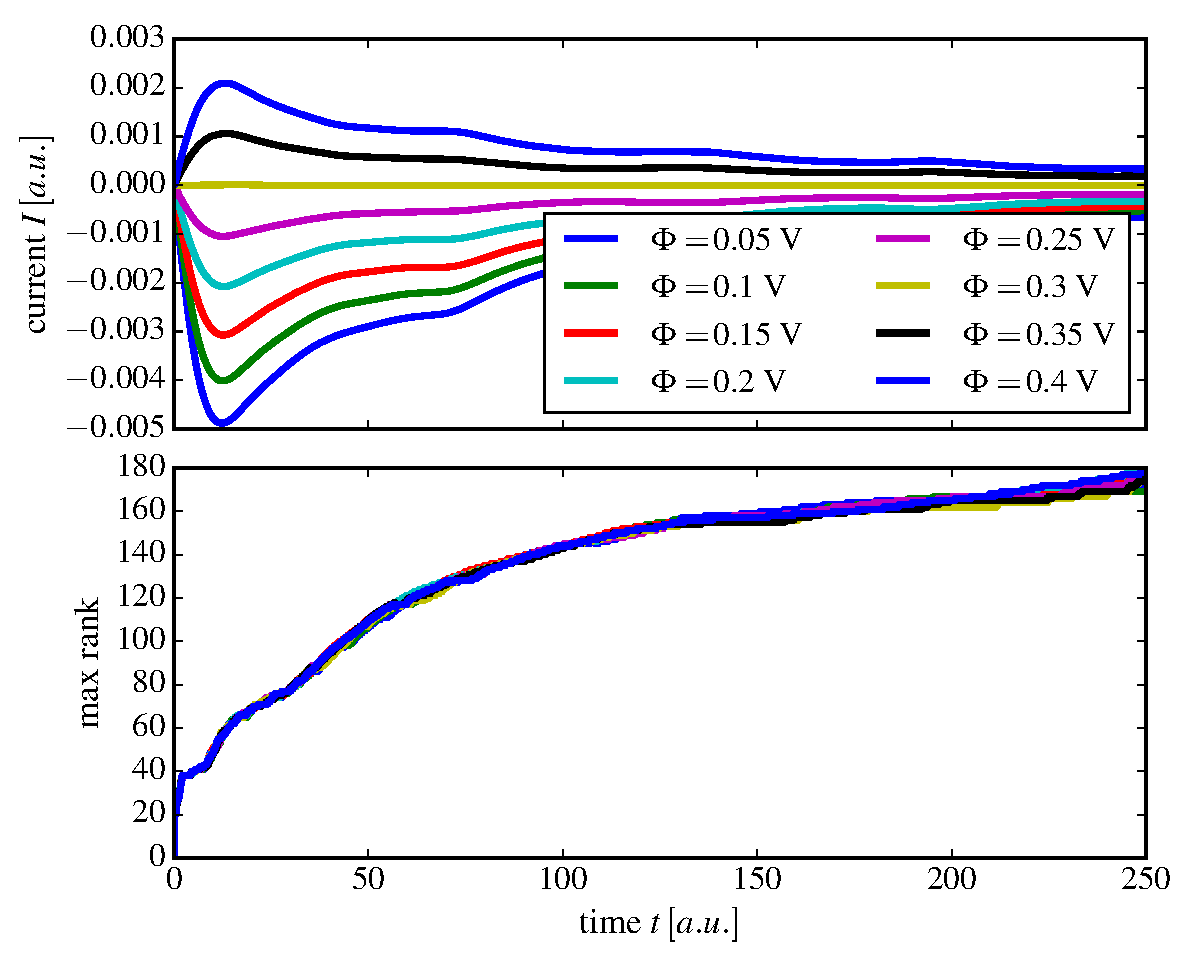
\includegraphics[width=0.7\textwidth]{figs/model_1_VVar_nv10.pdf}
	\caption{Dynamics of charge current and maximal rank for varying voltage for $n_\mathrm{vib}=10$.}
\end{figure}
\begin{figure}[!h]
	\centering
	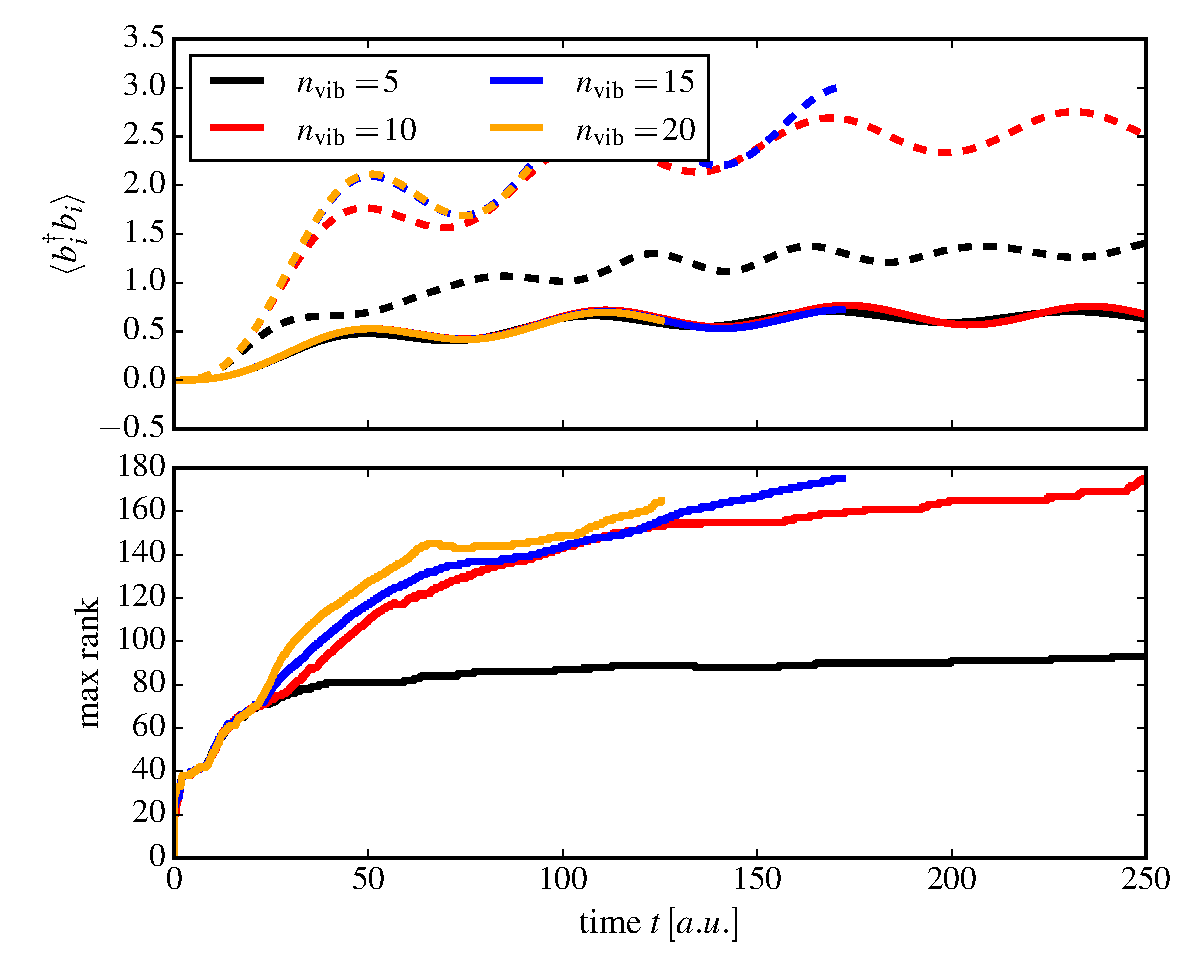
\includegraphics[width=0.7\textwidth]{figs/model_1_nvVar_V35.pdf}
	\caption{Dynamics of vibrational occupation number (bold: mode 1, dashed: mode 2) and maximal rank for varying vibrational basis states for $\Phi=\SI{0.35}{\volt}$.}
\end{figure}
\clearpage
\section{Model 2}
The second model has adiabatic coupling to the first mode and non-adiabatic coupling to the second mode
\begin{equation}
	H_1 = \varepsilon_0(d_1^\dagger d_1^\pdagger + d_2^\dagger d_2^\pdagger) +\sum_i\omega_i b_i^\dagger b_i^\pdagger + \lambda_1(b_1+b_1^\dagger)(d_1^\dagger d_1^\pdagger - d_2^\dagger d_2^\pdagger) +\lambda_2(b_2+b_2^\dagger)(d_1^\dagger d_2^\pdagger + d_2^\dagger d_1^\pdagger)
\end{equation}
\begin{figure}[!h]
	\centering
	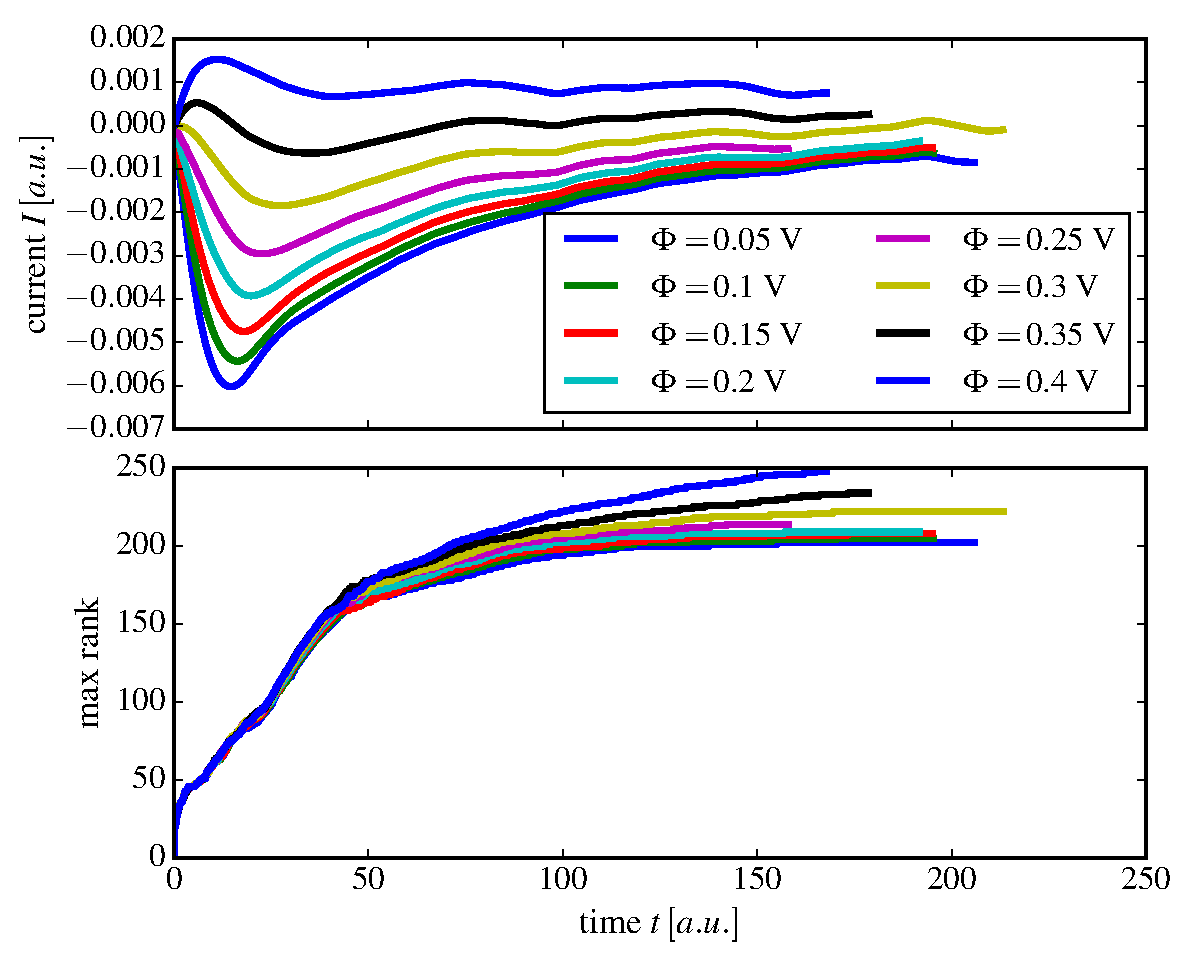
\includegraphics[width=0.7\textwidth]{figs/model_2_VVar_nv10.pdf}
	\caption{Dynamics of charge current and maximal rank for varying voltage for $n_\mathrm{vib}=10$.}
\end{figure}
\begin{figure}[!h]
	\centering
	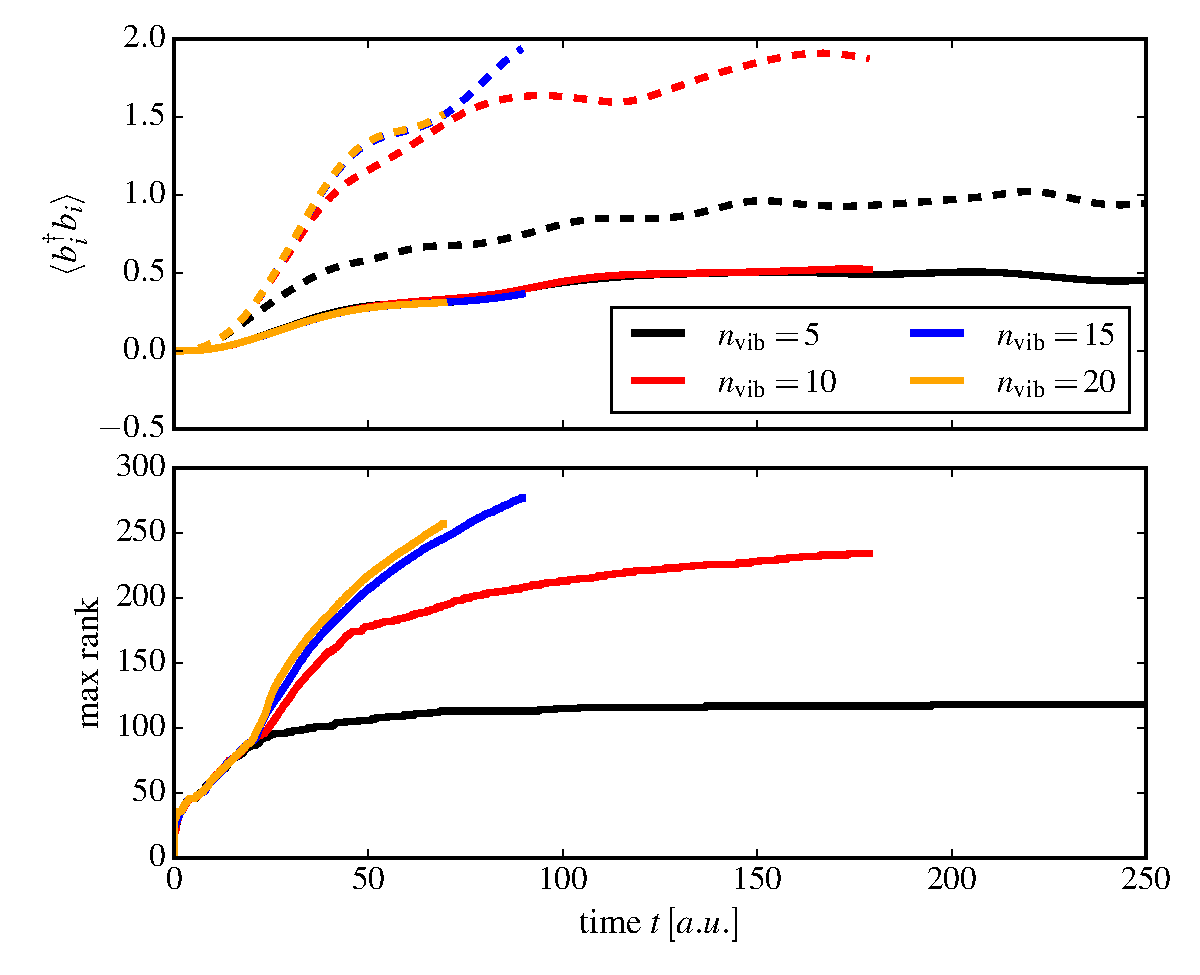
\includegraphics[width=0.7\textwidth]{figs/model_2_nvVar_V35.pdf}
	\caption{Dynamics of vibrational occupation number (bold: mode 1, dashed: mode 2) and maximal rank for varying vibrational basis states for $\Phi=\SI{0.35}{\volt}$.}
\end{figure}

\end{document}


